\section{Friday, June 28, 2019}

Today, we're going to discuss bits and bitwise operations. \\


Recall from last lecture that the negative representation of an integer can be obtained by inverting all of the bits and adding $1$. As an example, consider the number \texttt{01110}, which corresponds to the decimal number $15$. By inverting the bits and adding one, we see the number $-15$ can be represented as \texttt{10010}, and this can easily be verified for correctness by noting that \verb!01110 + 10010 = 00000!. 

\subsection{Review of Numeric Base Systems}
We should already be familiar with how to convert between two different bases. However, we can briefly recap:

\begin{itemize}
    \item To convert from base $10$ (what we are accustomed to) to binary, repeatedly divide the number by $2$, and keep track of the remainders. The binary representation of the number will be the remainders concatenated together in reverse-chronological order. 
    \item To convert from binary to base $10$, multiply the $i^{\text{th}}$ bit from the right (starting from $0$) by $2^{i}$. The desired number in base $10$ will be the sum of these powers. 
\end{itemize}

Consider the following conversion table:

\begin{center}
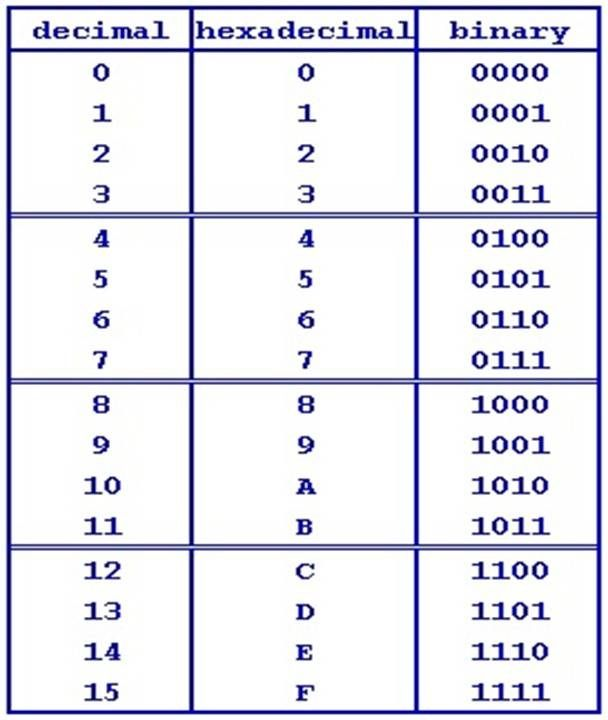
\includegraphics[width=5cm, height=7cm]{june28/table}
\label{conversiontable:1}
\end{center}

From the table above, it becomes clear that a single hexadecimal digit requires four bits for its representation. This matters because it allows us to quickly convert between hexadecimal and binary. Consider, for example, the hexadecimal number $55$. We can look at each hexadecimal digit, and we can write down the corresponding binary number with four bits to obtain $01010101$ as the equivalent binary representation. 


The \verb!printf()! command has a format specifier to print a number in hexadecimal (with the \verb!%X! specifier) or octal (with the \verb!%o! specifier). Moreover, the \verb!%08x! specifier can be used for printing unsigned integers as zero-padded, eight-digit hexadecimal numbers. However, there is no format specifier to print a number in binary. As an example, consider the following code segment: \newpage


\lstset{
caption=Hexadecimal Format Specifier}
\begin{center}
\lstinputlisting[language=c]{june28/june2801.c}\label{Hexadecimal Format Specifier}
\end{center}

The output of this program will be all hexadecimal numbers between $0$ and $32$, inclusive. There are additional zeroes added to the start of each number to ensure that each output is eight digits long. 



So, why do we specify that we want eight bytes, rather than some other number? In our system, an unsigned integer is $4$ bytes, or equivalently, $32$ bits (there are $8$ bits in a byte). Now since each hexadecimal number requires four bits, we require $32/4 = 8$ hexadecimal digits. 

As another example, suppose we're printing out a single character. There is $1$ byte, or equivalently, $8$ bits in a character. Hence, we require $8/4 = 2$ hexadecimal digits to print a character. \\

We can utilize the preceding fact and store a two-digit hexadecimal number as an unsigned character type. 


\subsection{Bitwise Operations}
First, we discuss bit shifting. \\


A bit shift moves each digit in a number's binary representation a specified number of places to the left or right. The left shift operator is written as \verb!<<!, whereas the right shift operator is written as \verb!>>!. The number that directly follows this operator specifies the number of places we wish to shift. 



As a basic example, consider the number $2$, which has binary representation \verb!0011!. If the variable $x$ were storing the value $2$, the statement \verb!x << 1! would return the value $4$ since the binary representation of \verb!x << 1! is \verb!0110! (note that an additional zero has been added at the end). The variable $x$ itself won't be updated from a bitshift. If we want to update the value of \verb!x!, we would have to instead write either \verb!x = x << 1! or \verb!x <<= 1!. Likewise, the statement \verb!x >> 1! would return the value $1$. Performing left and right shifts are equivalent to multiplying or dividing by powers of $2$. That is, a left shift by one multiplies by $2$, and the right shift divides by $2$ (note, however, that they are much faster than multiplying or dividing by $2$).



Some other bitwise operators include the logical operators of \verb!AND, OR, NOT!, and \verb!XOR!. These can be used in C with the binary operators \verb!&, |, ~,! and \verb!^!, respectively. We should already be familiar with these, but to recap, consider the numbers $5$ and $7$. The binary representation of these two numbers are \verb!0101! and \verb!0111!. Consequently, we see that \verb!5 & 7! returns $5$, \verb!5|7! returns $7$, \verb!~5! returns $10$, and \verb!5^7! returns $2$. \\

The identity for the \verb!AND! operator is $0$, and the identity for the \verb!OR! operator is $1$ (i.e. \verb!x&0 = x!, and \verb!x|1 = x!) \\


Note that all of these bitwise operations can also be applied to hexadecimal numbers (or rather, numbers in any base). It's just important to convert everything to binary first.  \\


\subsection{Bitmasking}

Why are bitwise operations important? We can use bitwise operations to perform \vocab{bitmasking}, ultimately allowing us to ``toggle'' or ``retrieve'' bits on and off. 


Consider a function that takes in an integer; say the input is \verb!1010!. If we want to always clear the second bit from the right, this function can simply return the user's input \verb!AND!'d with \verb!1101!, which will always result in a \verb!0! in the second bit. 
As another example, suppose we want to extract the second bit from the right of a given integer. Again, suppose the integer we're working with is \verb!1010!. We can \verb!AND! this number with \verb!0010!, which will clear everything except for our digit of interest. If the result is \verb!0!, the value of that digit is \verb!0!; otherwise, it is \verb!1!. 

Using \verb!AND! in conjunction with right shifts, we can write a program that counts the number of zeroes and ones in the bitwise representation of an integer.

In summary, \begin{itemize}
    \item We can clear bits by \verb!AND'!ing with $0$.
    \item We can check bits by \verb!AND!'ing with $1$.
    \item We can set bits by \verb!OR!'ing with $0$
    \item We can flip bits by \verb!XOR!'ing with $1$. 
\end{itemize}


Consider the following problem that can be solved with bitmasking: Given the hexadecimal number \verb!0xab! (which has binary representation \verb!1010 1011!), perform bitwise operations to make bits in positions $2$ to $4$ (from the left) equal to \verb!110!. 

The solution is to \verb!AND! with \verb!1000 1111! to clear the targeted bit positions, and finally \verb!OR! with \verb!0110 0000! to set them to what we desire. 


\subsection{Big Endian and Little Endian}

\vocab{Endianness} refers to how data is arranged in memory. It is dependent on the hardware we are working on (not the operating system). Endianness is important when we're working at the bit level. 

There are two types of endianness that we are concerned with: \begin{itemize}
    \item In \vocab{Big Endian} refers to how we typically visualize data. In this representation, there's a pointer that points to the most significant byte. 
    \item In \vocab{Little Endian}, the data is laid out in reverse-chronological order, and the pointer points to the least-significant byte.
\end{itemize}


Grace runs using little Endian.





